The first incarnation of NumPy was a package called Numeric, written in 1995
by Jim Hugunin, then completing his master's thesis at MIT.
Hugunin based his package on previous work by Jim Fulton,
then working at the US Geological Survey, and acknowledges
many others in his initial report of the package \cite{Hugunin-whitepaper}.
Later, Paul Dubois at Lawrence Livermore National Laboratory toke over the project
and funded the writing of the first
manual\footnote{https://conference.scipy.org/scipy2010/slides/travis\_oliphant\_keynote.pdf}.
Numeric provided an array object in Python, written in C, and linking to
standard fast implementations of linear algebra.
% https://stackoverflow.com/questions/26948776/where-did-the-term-broadcasting-come-from/26950256
% https://mail.python.org/pipermail/matrix-sig/1995-November/000143.html
% May want to mention Yorick here (origin of broadcasting idea; it is mentioned later)
% https://aip.scitation.org/doi/pdf/10.1063/1.4823451 
% https://aip.scitation.org/doi/pdf/10.1063/1.4822400

% S TODO: the first sentence below could flow a bit better
Around 2000, the Space Telescope Science Institute (STScI) software group wrote
a re-implementation of much of Numeric, called NumArray, to support their
need to work on large memory-mapped arrays and arrays of mixed data type
records \cite{STScI-slither}.
This briefly caused the Numeric and NumArray communities to diverge, until 2005,
when Travis Oliphant embarked upon a major rewrite that aimed to be a ``best of
both worlds'' unification of Numeric and NumArray \cite{oliphant2006guide}.
This merger resulted in NumPy.

NumPy now underpins almost every Python library that does scientific or
numerical computation, including SciPy\cite{virtanen2019scipy},
matplotlib\cite{hunter2007matplotlib}, pandas\cite{mckinney-proc-scipy-2010},
scikit-learn\cite{pedregosa2011scikit}, and
scikit-image\cite{vanderwalt2014scikit}.
NumPy consists of the $n$-dimensional array object along with utility functions
that operate on it.
Because of its inherent simplicity---being a pointer to memory with some
associated meta-data about shape, data-type, and so forth---the NumPy array is
the {\it de facto} exchange format for array data in Python.
The library has such widespread adoption that not only the array object but also its
{\it Application Programming Interface} (API) has become ubiquitous as
a language for tensor computation---witnessed by its use in popular
deep learning libraries such as PyTorch\cite{pytorch}.

% S: Maybe we want to emphasize Jax, which has rapidly become very popular

\section*{NumPy arrays}

\begin{figure*}
  \centering
  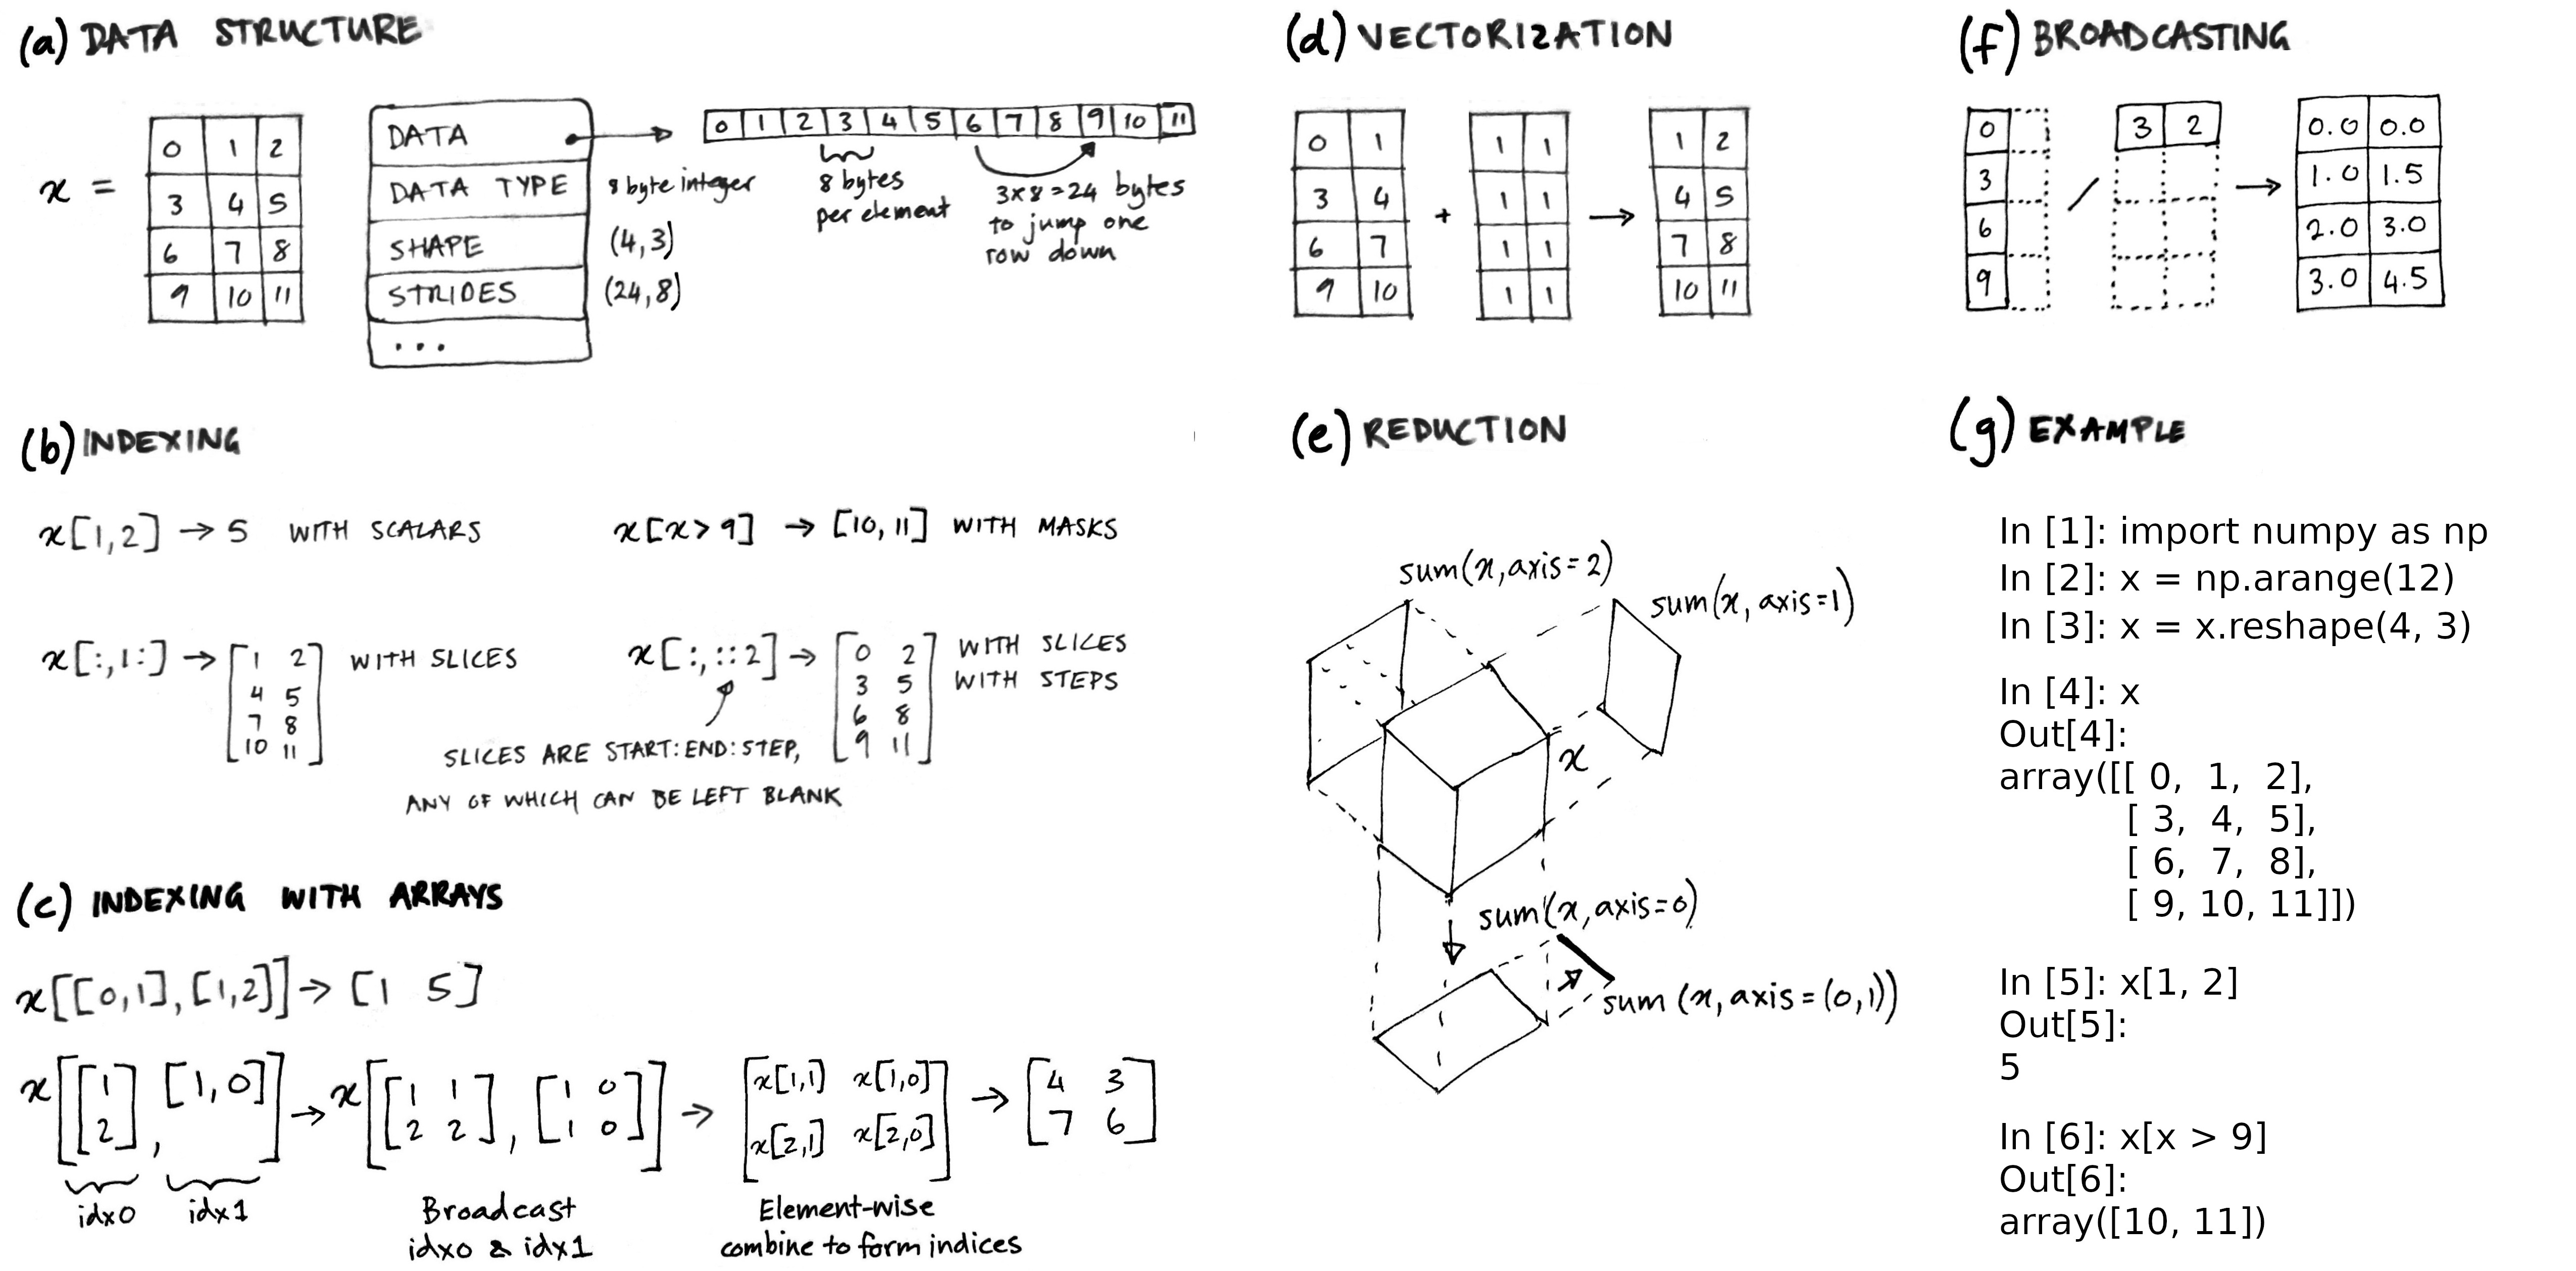
\includegraphics[width=\textwidth]{static/sketches/array-concepts}
  \caption{\fixme{PLACEHOLDER: This figure needs some text to describe
  it}
   }
  \label{fig:arrayconcepts}
\end{figure*}

The NumPy array is a structure that efficiently stores and accesses
$n$-dimensional array data\cite{vanderwalt2011numpy}.
The need for such a data structure arises often in science.
For instance, it may be used to store experimental measurements made at
discrete time intervals (1-D arrays), gray-level photographs (2-D arrays),
spectral measurement on a regular grid (3-D arrays), or color videos (4-D
arrays).

The NumPy array consists of a pointer to memory, along with meta-data used to
interpret the data stored there.
For example, while computer memory stores elements linearly and has no notion
of higher-dimensions, we can interpret it as $n$-dimensional arrays by also
providing its shape, strides (the number of bytes to advance in memory to skip
along rows, columns, etc.), and data-type.

Data types (dtypes for short) tell us more about the elements stored in a NumPy
array.
Arrays can hold, e.g., numerical data (of lower and higher precision), strings,
datetimes, or Python objects, each identified by its own dtype.

Once data is viewed as an $n$-dimensional array, more abstract operations such
as reductions (e.g., summation across columns), products, and so forth, are
defined (Figure~\ref{fig:reductions}).
Users predominantly interact with NumPy arrays using these operators and
associated utility functions through an easily readable high-level API
(Application Programming Interface).

Sometimes, it is desirable to combine arrays of different dimensions.
One may, for example, want to add a scalar to a vector, or scale each column of
an array by a specific scalar value.
This is done through {\em broadcasting}, where one of the arrays is virtually
duplicated (i.e., without copying any data in memory), so that the shapes of
the operands match.
Broadcasting is illustrated in Figure~\ref{fig:broadcasting}.

\begin{figure}
  \centering
  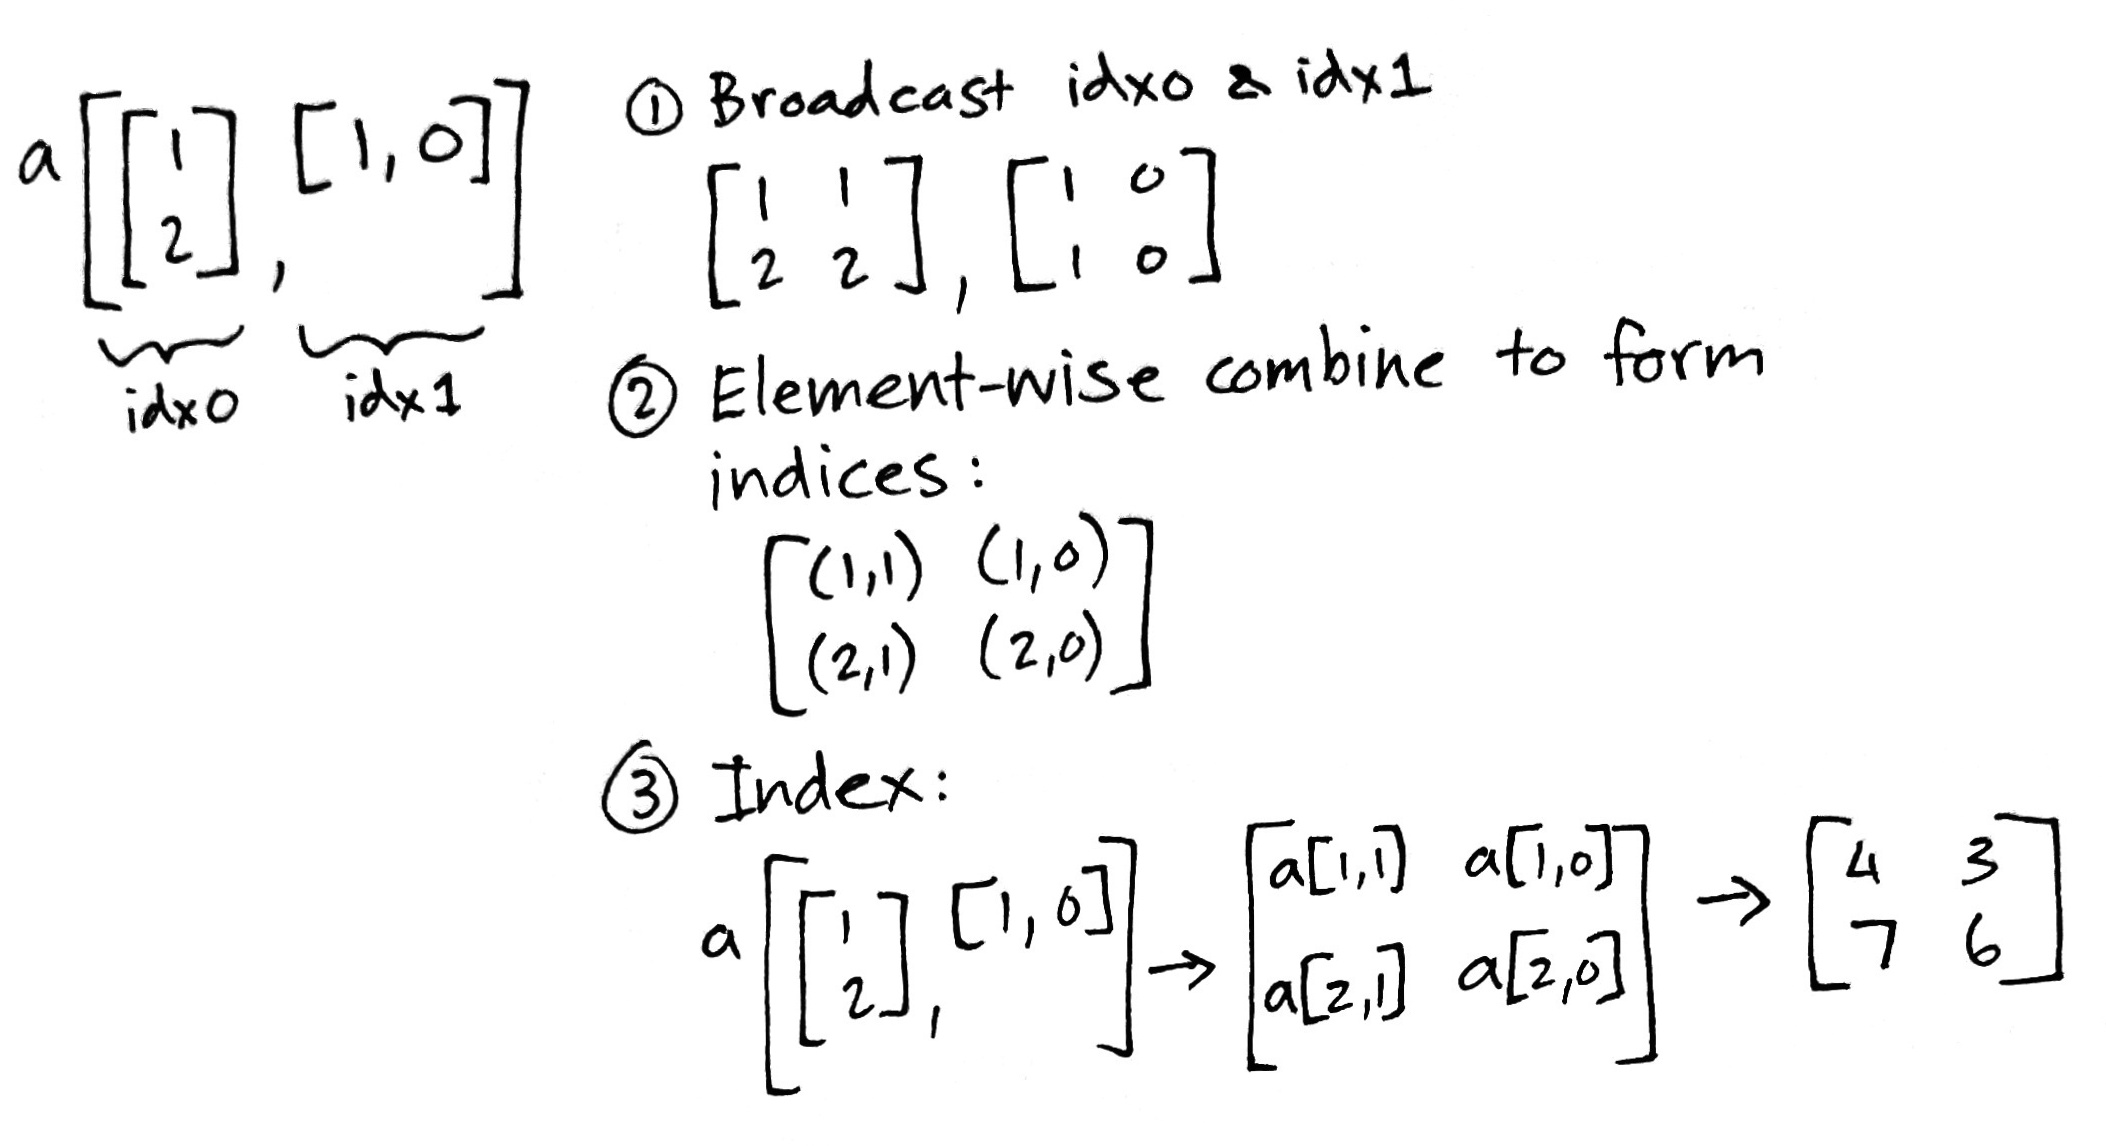
\includegraphics[width=\linewidth]{static/sketches/fancy-indexing}
  \caption{\fixme{Indexing using arrays, or ``fancy indexing''.}
   }
  \label{fig:broadcasting}
\end{figure}

NumPy include numerous functions that perform element-wise and reduction
operations on arrays, including arithmetic, statistics, and trigonometry.
They aim to loop over array elements near-optimally (taking into consideration,
e.g., strides, in order to best utilize the computer's fast cache memory), and
implement broadcasting.
Vectorized operations that would take many tens of lines to express in
languages such as C can often be implemented as a single, clear Python
expression.

\begin{figure}
  \centering
  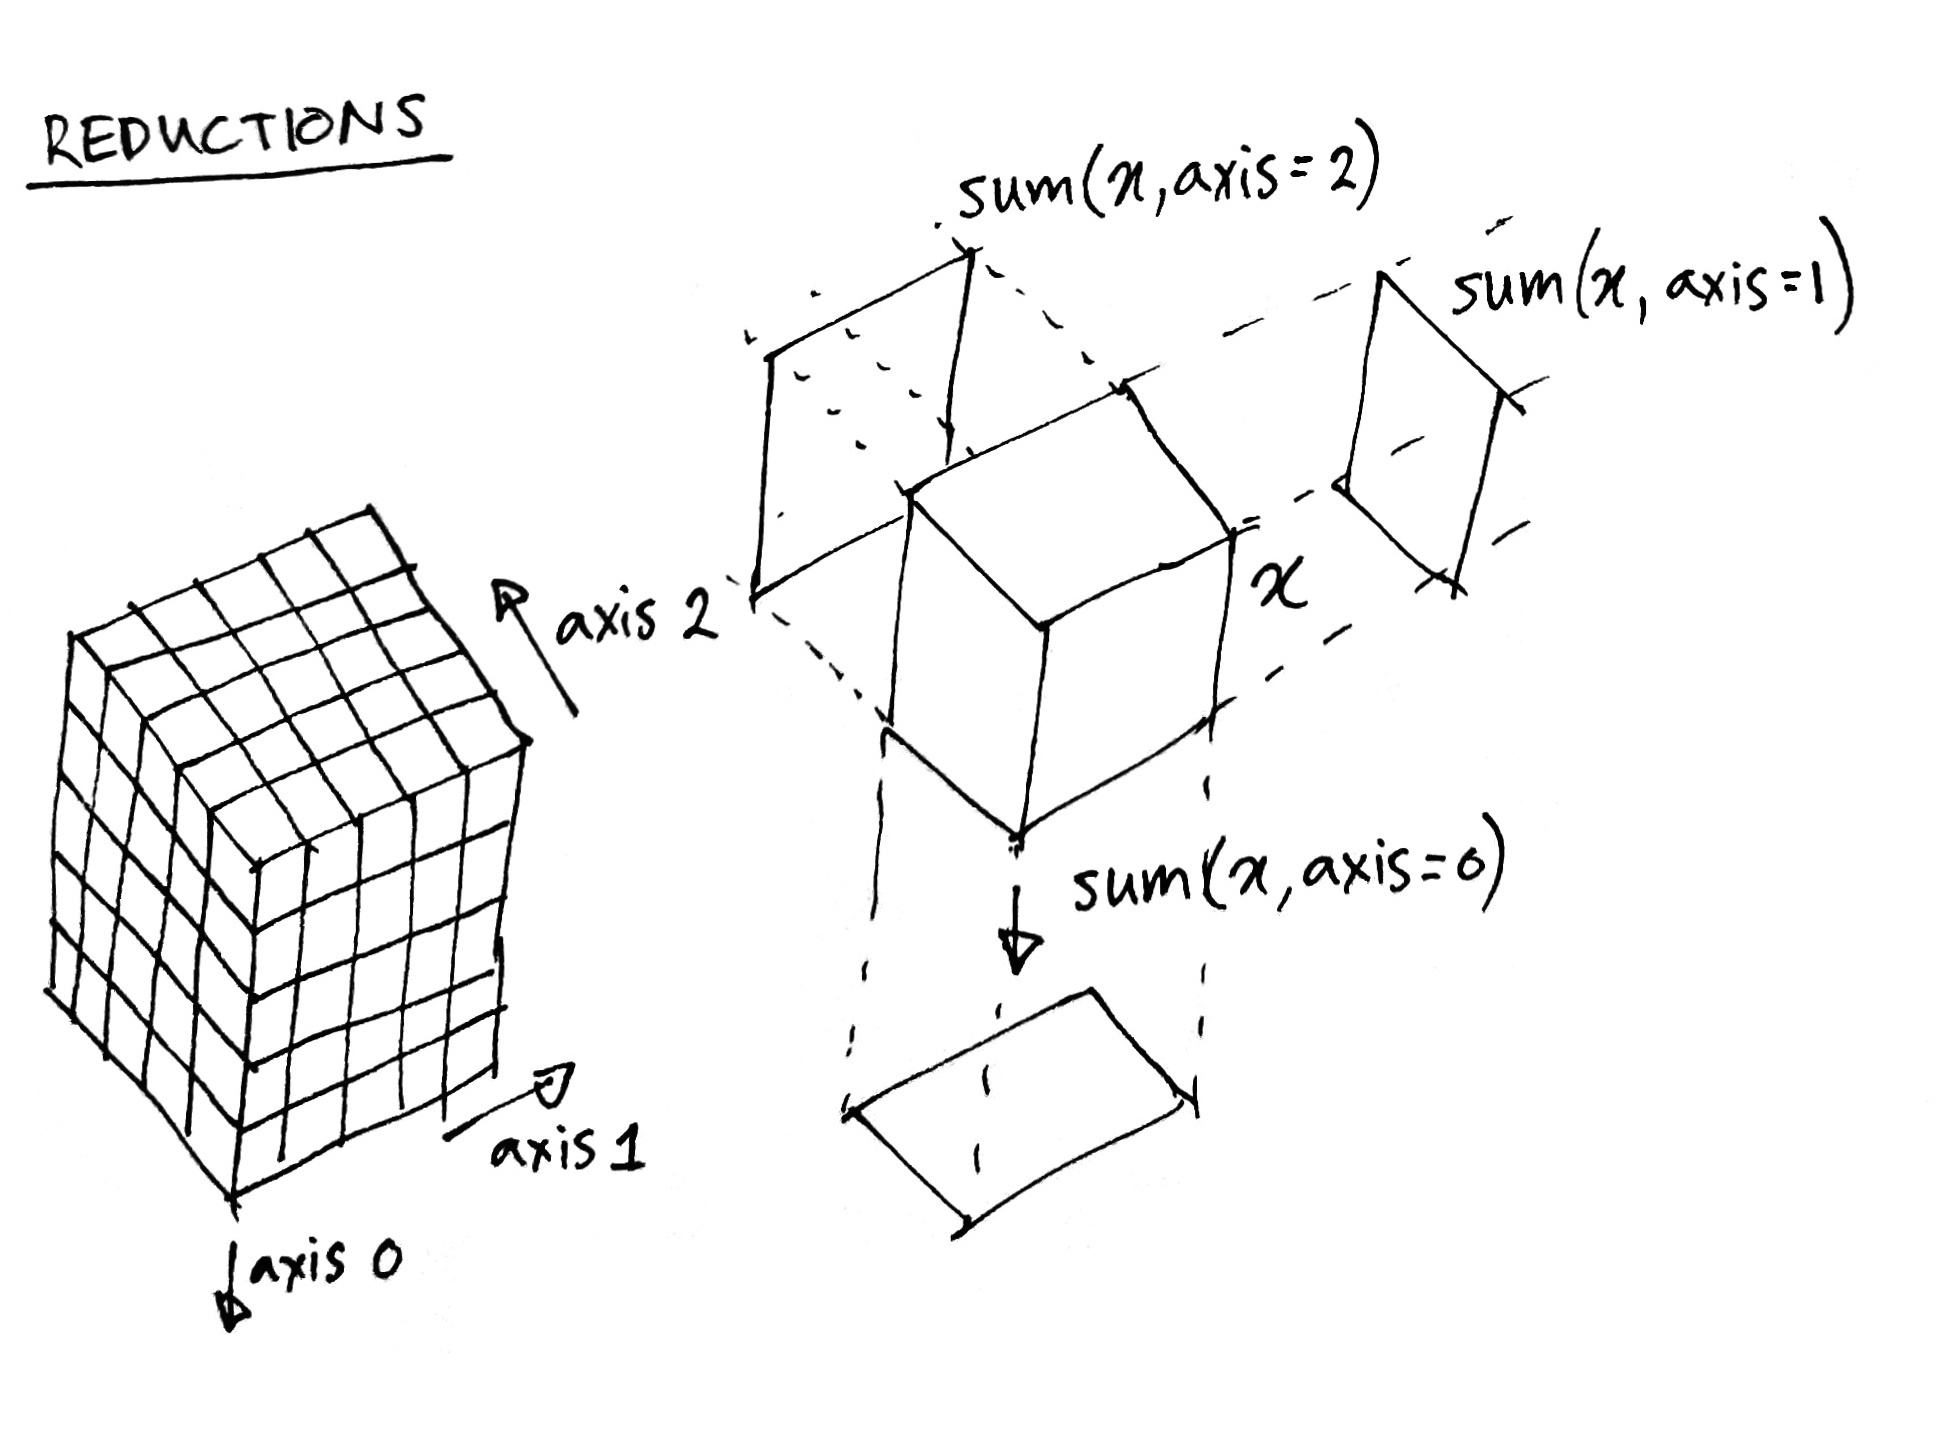
\includegraphics[width=\linewidth]{static/sketches/reductions}
  \caption{\fixme{Reducing an array along one of several axes.}
   }
  \label{fig:reductions}
\end{figure}

NumPy also provides support for accelerated linear algebra, and supports
several established backends such as OpenBLAS and Intel MKL.
Suppose the matrix \code{A} is a 2-d array and the vector \code{x} is a 1-d array.
Then \code{A @ x} computes the matrix-vector product $Ax$ and \code{x @ A} computes
the vector-matrix product $x^\top A$.
This matrix multiplication operation extends to higher-dimensions by treating
the array as a stack of matrices.

In addition, NumPy provides a large collection of utility functions for
creating, reshaping, concatenating, and padding arrays; for searching, sorting
and counting data in arrays; and for reading and writing files.
It provides extensive support for generating pseudorandom numbers and includes
an assortment of probability distributions.


\section*{Changing computational landscape}

\fixme{Ralf will take a first pass on the section on 1/12.}

\fixme{The idea here is something like:  classic numpy (as described above)
was built to solve previous problems; new problems have arisen as
the computational landscape has changed; new hardware, new languages,
new problems; as a result np's role has changed; it is a foundational
tool widely-used not a specialist tool used by scientist developers;
many array-like libraries for various uses and np is serving as
a standard)}

NumPy was initially developed by students, faculty, and researchers in their
spare time to provide a modern array computation library for Python.
They were influenced by their experiences with powerful interactive programming
languages for scientific computing like Yorick \cite{munro1995using} as well
as commercial languages like IDL and Matlab.
Often they developed code to solve their own or their colleagues' problems.

As Python's popularity for scientific computing, data science, and machine
learning increased, many new use cases arose.

- GPUs

- distributed computing

- other languages w/ arrays

- massive explosion in data science, machine learning, and artificial intelligence

NumPy also went from a small community of mostly expert users to
one of the most widely used foundations of the scientific Python
ecosystem.
Now the user base is very different....
% maybe worth a sentence or two about how we are working on web and
% user docs to make it easier for new users to get started...

\section*{Interoperability and extensibility}

\begin{figure*}
  \centering
  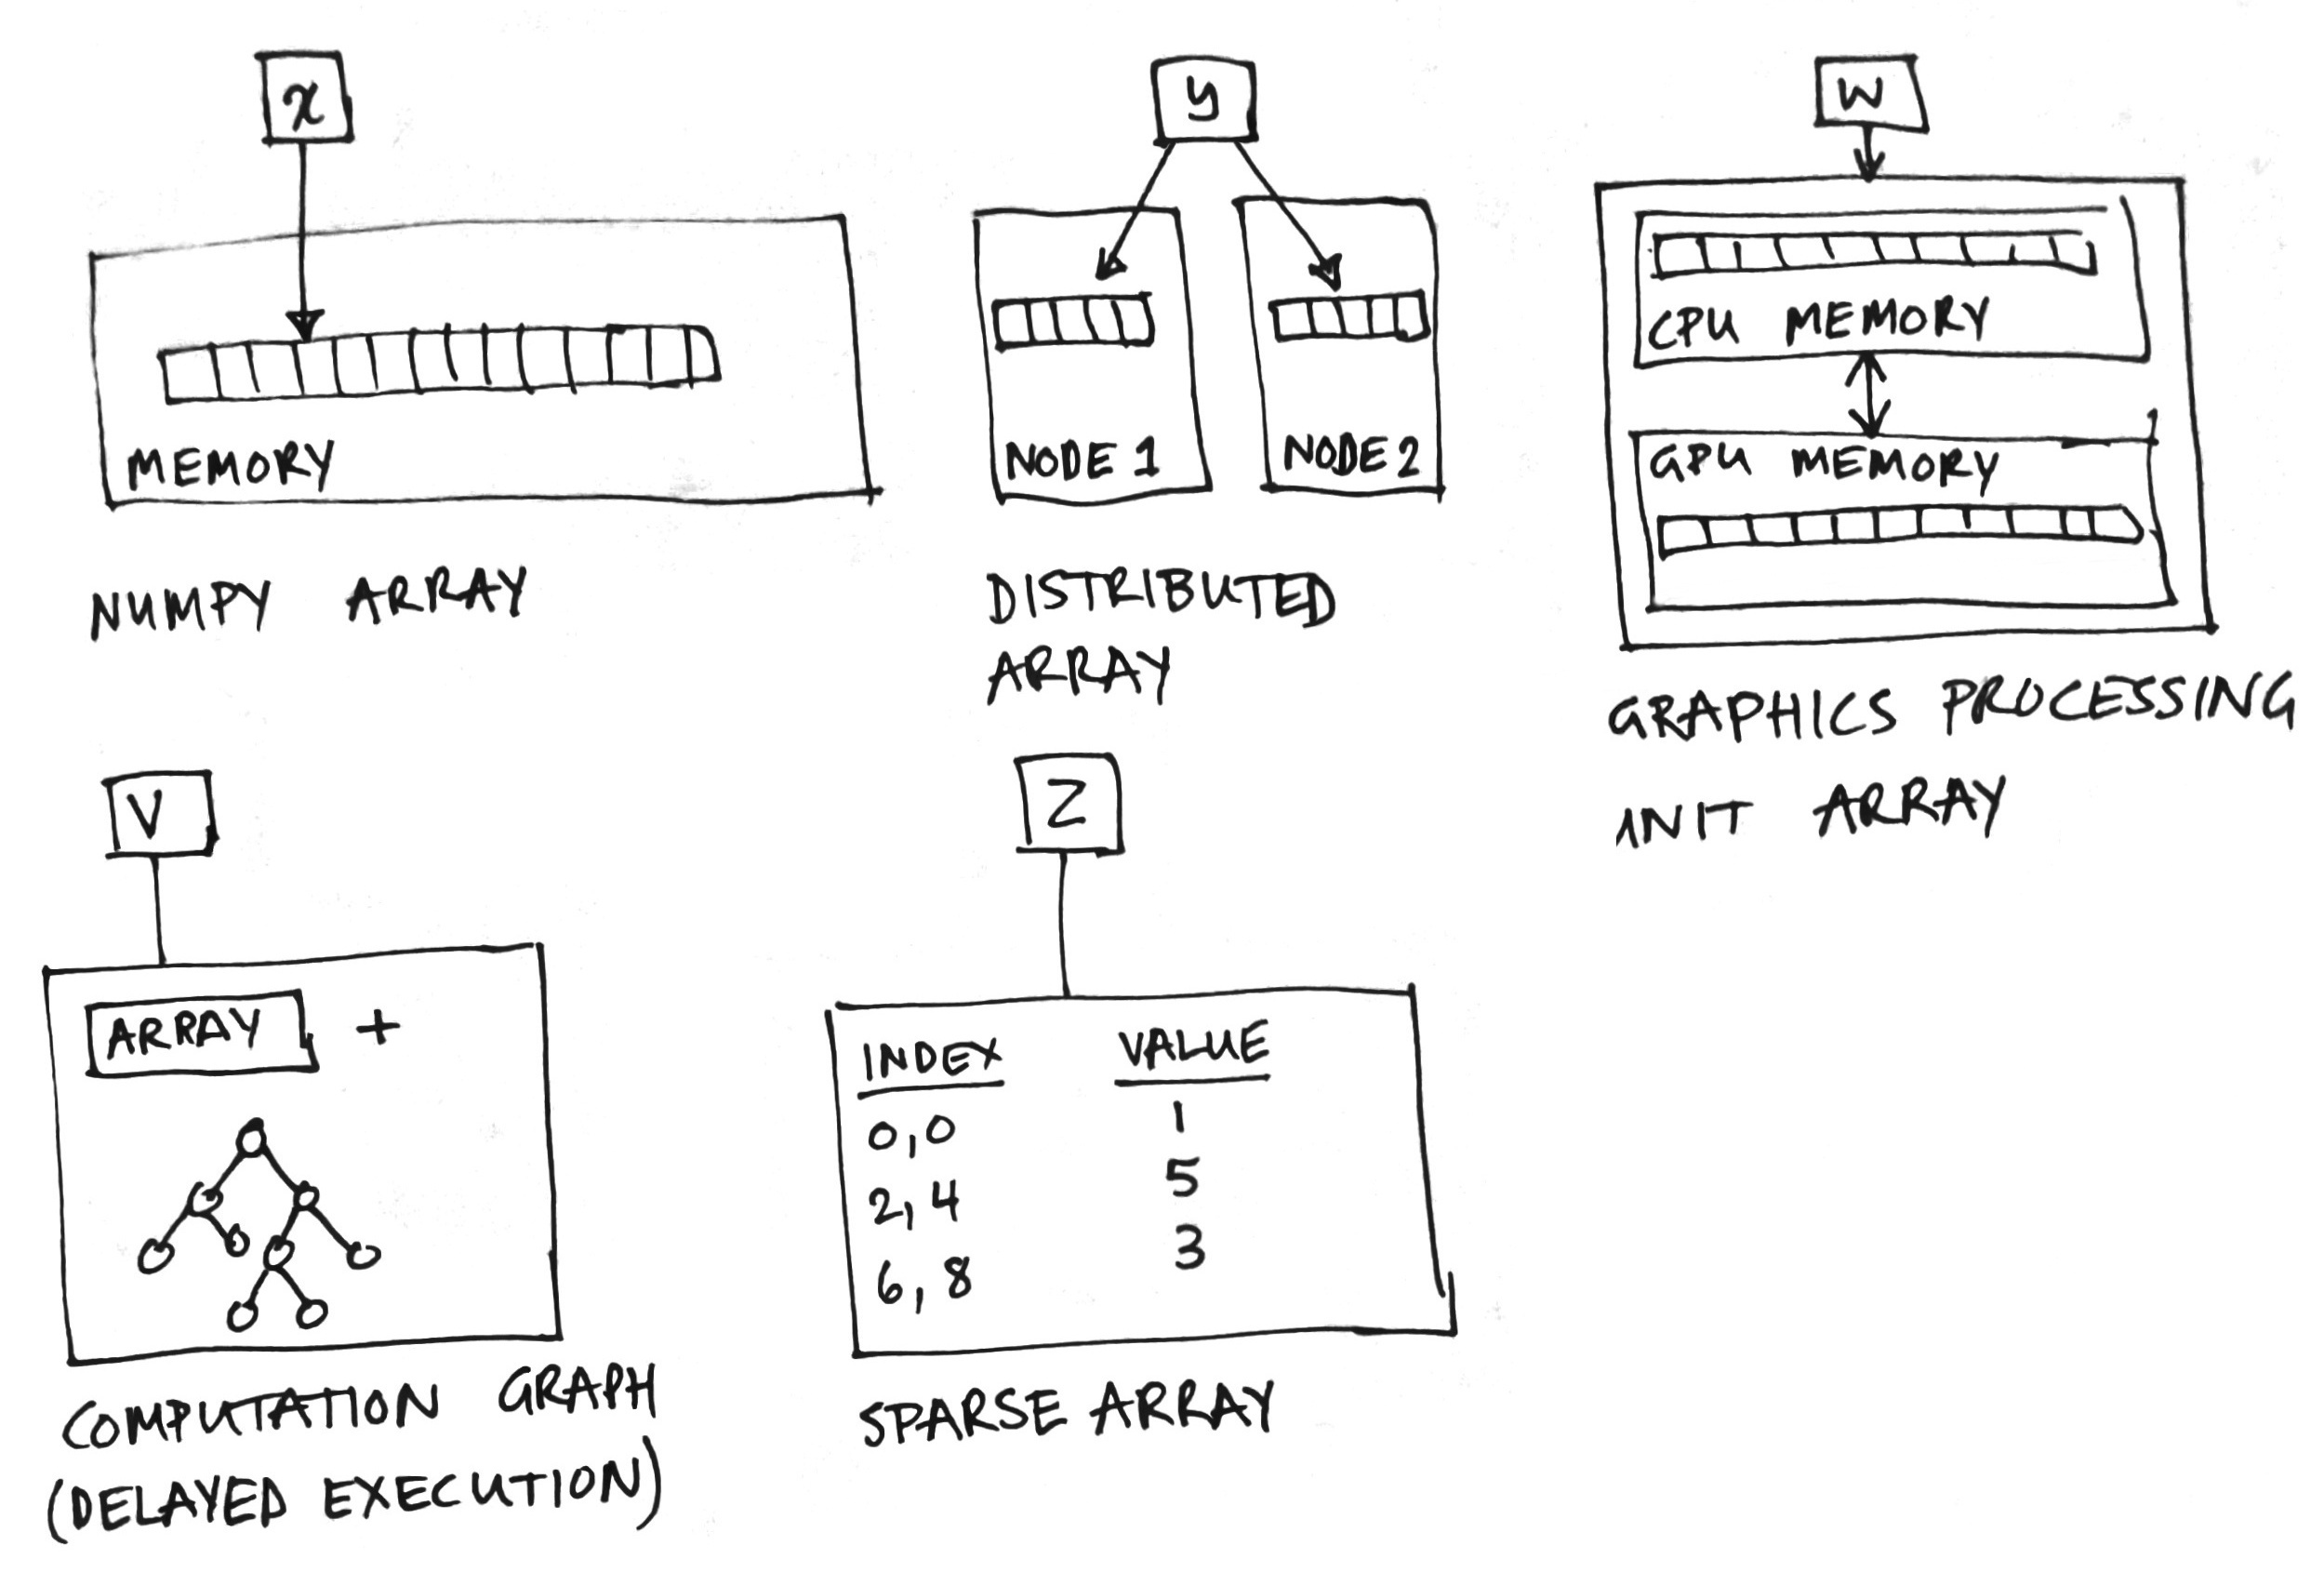
\includegraphics[width=0.8\textwidth]{static/sketches/duck-arrays}
  \caption{\fixme{Examples of so-called ``duck arrays'': arrays
  implemented by another library that behave like NumPy arrays, and
  support NumPy operations.  Through protocols, it is possible to have
  a call such as $\cos(\cdot)$ succeed on each of these.}}
  \label{fig:duck-arrays}
\end{figure*}


% https://numpy.org/neps/nep-0016-abstract-array.html
% https://numpy.org/neps/nep-0018-array-function-protocol.html
% https://numpy.org/neps/nep-0022-ndarray-duck-typing-overview.html
% https://numpy.org/neps/nep-0030-duck-array-protocol.html
% https://github.com/numpy/numpy/blob/a111b551ae940d7d5f8523fef1cf3589c6ba00a0/doc/neps/nep-0033-extensible-dtypes.rst
% https://numpy.org/neps/nep-0037-array-module.html

A vast number of projects are built on NumPy;
these projects are consumers of the NumPy API.
Over the last several years, a growing number of projects are providers of
a \emph{NumPy-like API} and array objects targeting audiences with specialized
needs beyond NumPy's capabilities (Figure~\ref{fig:duck-arrays}).
For example, the NumPy API is implemented by several popular tensor computation
libraries including CuPy\footnote{\url{https://cupy.chainer.org/}},
JAX\footnote{\url{https://jax.readthedocs.io/en/latest/jax.numpy.html}},
and Apache MXNet\footnote{\url{https://numpy.mxnet.io/}}.
PyTorch\footnote{\url{https://pytorch.org/tutorials/beginner/blitz/tensor\_tutorial.html}}
and Tensorflow\footnote{\url{https://www.tensorflow.org/tutorials/customization/basics}}
provide tensor APIs with NumPy-inspired semantics.
It is also implemented in packages that support sparse arrays
such as \code{scipy.sparse} and \code{pydata.sparse}.
Another notable example is Dask, a library for parallel computing in
Python.  Dask adopts the NumPy API and therefore presents a familiar
interface to existing NumPy users, while adding powerful abilities to
parallelize and distribute tasks.

\fixme{Similarly there are many projects that build on top of the NumPy API for
labeled and indexed arrays (XArray), automatic differentiation (Autograd,
Tangent), masked arrays (numpy.ma), physical units (astropy.units, pint, unyt),
etc. that add additional functionality on top of the NumPy API. Most of these
project also implement a close variation of NumPy’s level high API.}

The multitude of specialized projects creates the difficulty that consumers
of these NumPy-like APIs write code specific to a single project and do not support
all of the above array providers.
This is a burden for users relying on the specialized array-like, since
a tool they need may not work for them.
It also creates new challenges for end-users who need to transition
from NumPy to a more specialized array.
The growing multitude of specialized projects with NumPy-like APIs threatened
to again fracture the scientific Python community.

\fixme{We would like to be able to use these libraries together, for example we would
like to be able to place a CuPy array within XArray, or perform automatic
differentiation on Dask array code. This would be easier to accomplish if code
written for NumPy ndarrays could also be used by other NumPy-like projects.}

To address these issues NumPy has the goal of providing the fundamental
API for \emph{interoperability} between the various NumPy-like APIs.

For example, a new array protocol was implemented that allows NumPy to consume
array-like objects produced by libraries outside of NumPy.  When asking NumPy
to, e.g., sum such an array, instead of attempting that operation itself, NumPy
requests the original array to complete the computation.  This means that the
NumPy API---the syntax for interacting with arrays---can still be used, but now
with a library that supports GPUs, does distributed computation processing, or
stores data in the cloud.

Another ongoing example is a redesign of the data type system.
While the majority of users rely only on numerical dtypes, there are a
multitude of use cases for which the current implementation is unsuited, such
as physical units\cite{astropy,Goldbaum2018,pint}, geometrical
objects\cite{pygeos}, and automatic differentiation\cite{pyadolc}.
The proposed overhaul of the datatype system will make it behave consistently
and will simplify the creation of custom dtypes, both in C and in Python.


\section*{Discussion}

% aka why is this so successful
% some sense of ongoing work / future directions


The creation of NumPy spurred renewed development in the larger scientific
Python ecosystem and heralded the current era of wide-spread use of Python for
scientific computing.
There were several factors that allowed this rapid growth
and successful development.

Hugunin identified the first factor in his initial description of the Numeric
package \cite{Hugunin-whitepaper}.  Numerical computing is usually one
component of a larger programming task, therefore:
\begin{quote}
    Rather than trying to retrofit an existing numerical language to support
    the wealth of features found in a powerful, modern, general-purpose
    programming language, it makes much more sense to attack the problem from
    the other direction and add the features of a powerful numerical
    programming language to Python.
\end{quote}
Python is already a good choice for many standard programming tasks such as
cleaning data, interacting with web resources and parsing text.  It has a wide
range of libraries for many different tasks. Adding fast array operations and
linear algebra allows the scientist to do all their work with within the same
language---and one that has the advantage of being famously easy to learn and
teach.

The second factor flows from Python's nature as an open-source language,
embedded within the open-source community.  Python attracts developers who like
to build and contribute.  As a result, NumPy has always been a library that was
developed by scientists in order to do their work.  Commercial specialist
numerical languages can encourage consumer-users, who pick up a tool and use
it, but do not expect to contribute to development%<-sentence a bit tough to parse.
In contrast, NumPy often
attracts user-developers, who want to work with NumPy, and are prepared to fix
and extend the library as they work. User-developers have been the fundamental
force in developing NumPy, and shaping it into a library that has been refined
in the furnace of practical scientific work.

The third factor is much like the second: 
%a culture in Python that concentrates
%on high quality of code and distribution.  Because Python is open-source, it has
%a strong culture of contribution, and therefore, of using tools and process to
%improve collaborative software development, such as distributed version
%control, code review, and automated testing.  These have allowed the project to
%scale safely as it attracted more users and developers, even though these
%developers rarely came to the project with training in software engineering.
the project has strong culture of using software-engineering practice to
improve collaboration and reduce error \cite{millman2014developing}.
The NumPy team was early in adopting distributed
revision control and code review to improve collaboration on code, and
continuous testing that runs a large battery of automated tests for every proposed
change to NumPy.
The project has comprehensive, high-quality documentation,
integrated with the source
code\cite{vanderwalt2008scipy,harrington2008scipy,harrington2009scipy}. 

Lastly, we believe NumPy has benefited greatly from a well-chosen application
programming interface (API).  Scientific and numerical programming needs to be
fast, and scale to very large datasets.  The NumPy API defines a simple wrapper
for data in memory so it can be represented as a one- or multi-dimensional
array.  The simplicity of this wrapper has made it very successful as a
standard way of representing arrays in memory, and has made it relatively easy
for other libraries to develop fast and memory-efficient compiled code, usually
in C or Fortran, that can manipulate these arrays and pass them back to Python.
This has been a large factor in the growth of numerical computing libraries
around NumPy and Python.

% S: I think two issues are conflated here: the simple underlying memory model, and the API.  The API has developed organically, while the underlying memory model is a design decision that shapes much of how the rest of the library was built.

% S:
%
% Thinking about enabling factors, I'd characterize them into three categories:
%
% - Practical
% - Philosophical
% - Social
%
% E.g., practical: reason why we use Python (learn one language for everything); students don't have money, so want to avoid impracticalities of license dongles/servers, etc.
%
% Philosophical: science should be open, transparent; our software should be controlled by scientists, not designers that we don't have access to
%
% Social: joy of building these things together, friendly welcome into the community for many of us---appreciation of our work and hours
%

